% Continuum Mechanics

\vskip -0.4in
\section{Introduction}
 % <<<
Before discussing the Navier-Stokes equations,
we must first discuss some basic kinematic and dynamical ideas in mechanics necessary to describe a continuum
model of a fluid. It will turn out that the incompressible Navier-Stokes equations are a quite simple modification of
the standard momentum conservation law of continuum mechanics.
The equations of motion (for example, resulting from $F = ma$) for a finite dimensional system
governed by Newtonian mechanics are usually ordinary differential equations.
The equations of motion for a system in continuum mechanics (for exampling, resulting from the Cauchy momentum equation, described soon),
are partial differential equations. However, more fundamental is the resulting set of \textit{integral conservation laws},
from which a corresponding system of partial differential equations can be derived.
% Although the focus later will be on fluid mechanics, a large set of fundamental concepts of solid and fluid mechanics
% are the same. The key distinction appears when one focuses on displacements and materials with ``shear strength'' (solids)  versus flows
% and materials with no shear strength (common fluids).
% >>>

\vskip -0.4in
\section{Transport}
\begin{figure}[H]
\centerline{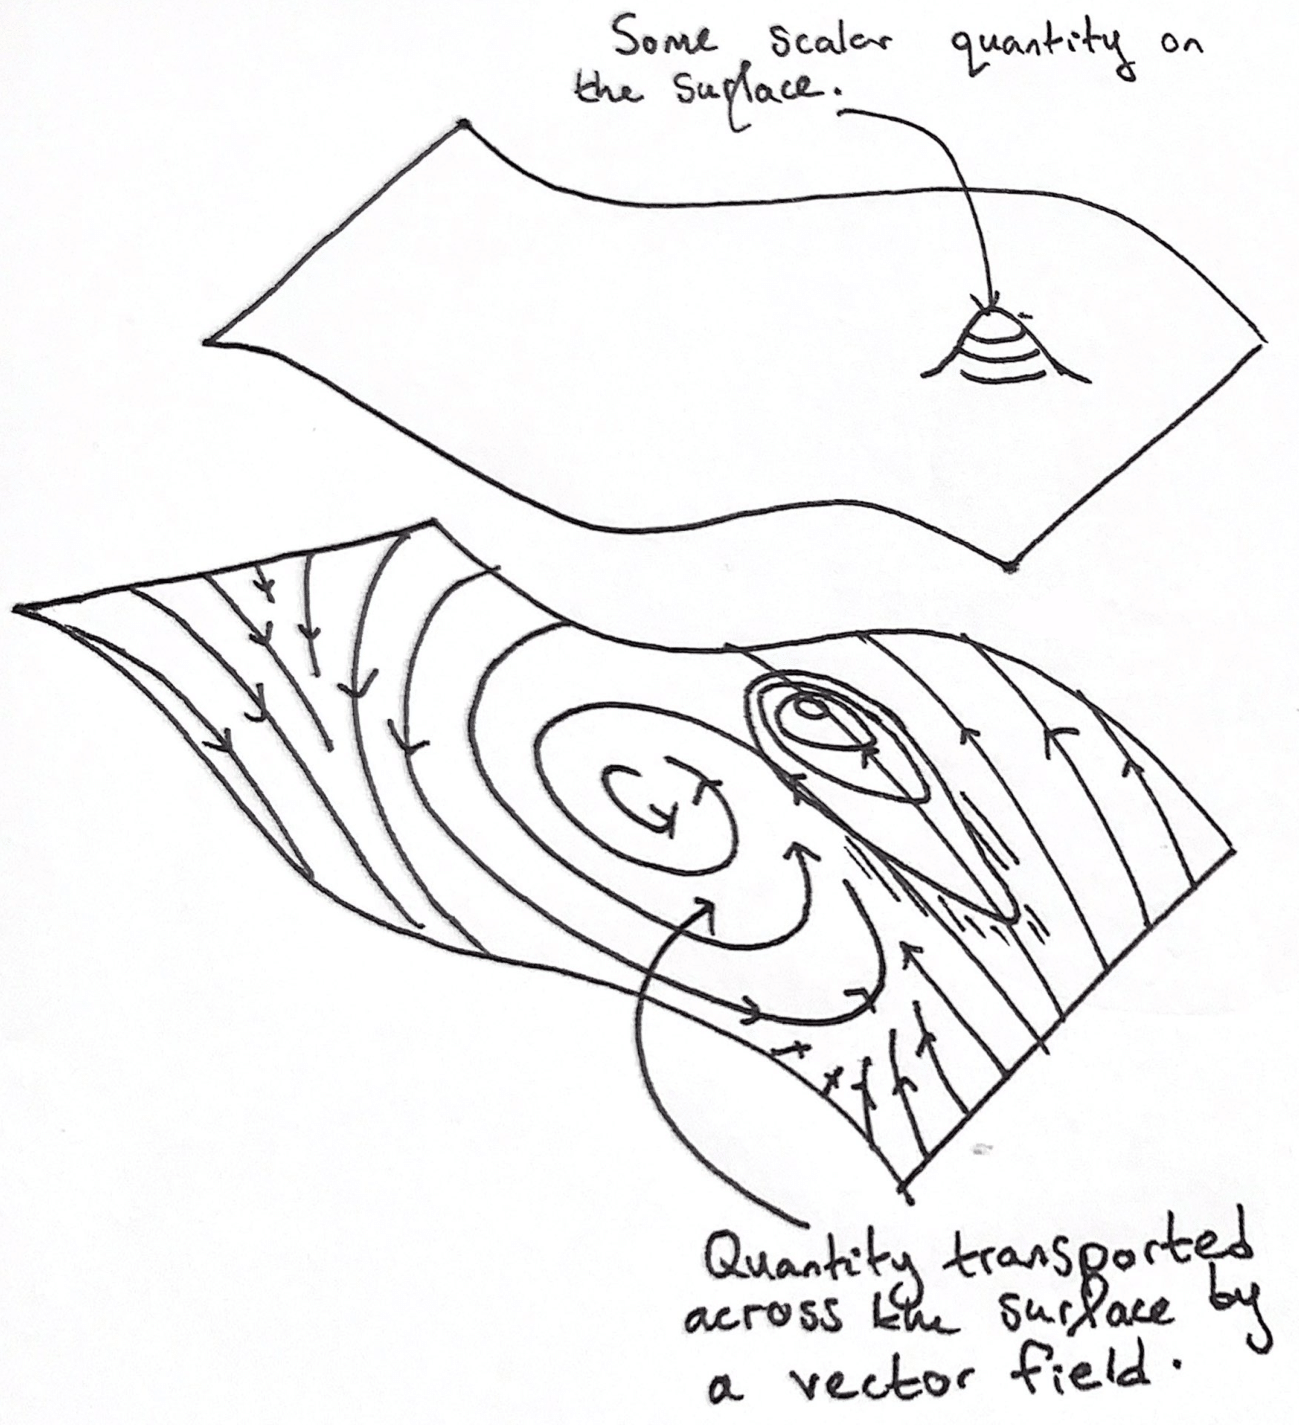
\includegraphics[width=0.45\textwidth]{figures/sketches/transport.png}}
\caption{A distributed quantity transporting across a continuum.}
\label{sketch_transport}
\end{figure}
% <<<
% Introduction
% <<<
Before considering continuum processes in the framework of Newtonian and Lagrangian mechanics, we will look at a fundamental notion of a ``motion''
of a point in a function space. Many continuum models in physics, such as the heat equation,
Maxwell's equations, and the equations of fluid motion, are formed by \textit{conservation equations}. These laws posit that the
evolution of the state (represented by a function) is
due to the transport of the quantity that the function measures, which is either pushed around (by some flux either predetermined or dependent on the current state),
introduced into the system at sources, or leaves the system at sinks.
This transport process is sketched above, in figure \ref{sketch_transport}.
% (figure of some manifold embedded in space, and some vector field pushing quantity around)
% \begin{figure}[H]
% \centerline{\includegraphics[angle=90,page=11,width=0.44\linewidth]{figures/2.pdf}}
% \caption{Thing}
% \label{sketch_transport}
% \end{figure}
We consider here the transport of quantities (scalar, vector, and tensor) on a general finite-dimensional manifold $M$,
colloquially called ``the continuum''. All transporting vector fields (``flux functions'') are considered to be tangent to this manifold $M$.
% >>>
\subsection{Continuity equations and conservation laws}\label{conservation_laws}
% <<<
\subsubsection{The integral form of a continuity equation}
Consider some spatial quantity $\phi$ on $M$ and a flux function $j$ which by which
this quantity flows around $M$. For clarity, we will begin by specializing $\phi$ to be a scalar, although later we will find it useful to
transport vector quantities such as momentum. By definition we want this flux function to just push quantity around.
The entering and exiting of quantity into and out of the system is determined by some arbitrary source function $s$ (of the same kind as $\phi$). These variables are related by the
conservation condition
\begin{equation}\label{continuity_equation}
    \frac{d}{dt} \int_{\Omega_0} \phi\,dx = \int_{\Omega_0} s\,dx + \int_{\pomn} \phi j \cdot \left(-\hat{n}\right)\,dx
\end{equation}
for arbitrary control volumes $\Omega_0$ in the continuum. The term $-\hat{n}$ denotes the inward-pointing normal to the boundary of the control volume. This simply says that the change in the total quantity in the fixed control volume is accounted for exactly by that quantity pushed through the boundary by the flux function $j$, and the internal sources and sinks of quantity $s$.
% --- $s_B$ as a boundary term? Why introduce this? Seems to be needed for the derivation of surface forces.
% (--- It may be useful to add $s_G$ as a boundary source term at $\pomn \cap \pom$ so Dirac delta ideas don't need to be used for non-fluxed boundary source (or, for example, the domain might be a subdomain where the transported function is unknown outside, so the term is introduced through $s_G$.))

\subsubsection{The differential form of a continuity equation}
A common technique in continuum modelling is the use of Stokes' theorem to simplify integral expressions.
Stokes' theorem and its specialisations (such as the divergence theorem and Green's theorem) are really \textit{definitions} of pointwise quantities
such as the divergence and curl as limits of these integral expressions for arbitrarily small regions.

The idea is that a space can be broken into many little pieces. If an integral equation holds over small regions, by linearity,
the integral equation will hold over larger elements, formed by combining the smaller elements.
If the elements are made ``infinitely small'',
then the result is a \textit{differential equation} which holds at each point. There are some analytical issues here, but
the hope is that if the differential equation holds at each point, the integral equation will hold over each control volume thought of
as an aggregate of infinitely small pieces.
For example, if $\Omega_\epsilon$ is a ball of radius $\epsilon$ around
a point $x^* \in M$, then the divergence can be defined as
\begin{equation}
    \nabla\cdot v (x^*) \coloneqq \lim_{\epsilon \rightarrow 0} \frac{1}{\text{Area}(\pom_\epsilon)}\int_{\pom_\epsilon}v\cdot\hat{n}\,dx.
\end{equation}
% \begin{equation}
%     \int_{\pom}v\cdot \hat{n}\,dx = \sum_{i\in\mathcal{I}}\int_{\pom_i}v\cdot \hat{n}\,dx.
% \end{equation}
% \begin{equation}
%     \int_{\pom}v\cdot \hat{n}\,dx = \int_\om \left[\lim_{\epsilon \rightarrow 0}\frac{1}{\pom_{x,\epsilon}}\int_{\pom_{x,\epsilon}}v\cdot\hat{n}\,dx^\prime\right]\,dx.
% \end{equation}
% 
% 
Equation \eqref{continuity_equation} becomes
\begin{equation}\label{continuity_equation_differential}
    \Part{\phi}{t} = s - \nabla\cdot (\phi j)
\end{equation}
assuming that $\phi j$ is sufficiently differentiable such that the limiting integral exists.
Continuity relations are most naturally expressed in form \eqref{continuity_equation}, while the form
\eqref{continuity_equation_differential} may be more useful for techniques such as finite differences.
Later, when we discuss numerical methods for solving continuum models, we will not take this route. The methods of interest, \textit{Galerkin} methods,
work naturally with the integral form \eqref{continuity_equation}.
It will be seen later that some constructions in the presentation of Galerkin methods, such as the ``weak form'' of a PDE, simply undo the differentialisation
(for example \eqref{continuity_equation_differential}) of the original integral form of physical PDEs (for example \eqref{continuity_equation}).
% (--- note: Maybe not exactly, as the integral conservation is quantified over regions, while the weak form is quantified over test functions,
% which still need to be sufficiently differentiabile. But I think that this must express the same continuity relation.)
% >>>
\subsection{The Reynolds transport theorem}
% <<<
\subsubsection{The integral form of Reynolds transport}
With our integral formulation of a continuity relation \eqref{continuity_equation}, the control volume $\Omega_0$ is fixed.
We may change our perspective by considering, in addition to the flux function $j$ (which transports quantity $\phi$), another
vector field $\hat{u}$ which will transport our control volume $\Omega_0$. The rate of change of some time-dependent quantity $\gamma$ in this
\textit{moving} control volume is expressed as
\begin{equation}\label{reynolds_rate_of_change}
    \frac{d}{dt}\int_{\Omega_0(t)}\gamma\,dx,
\end{equation}
where $\Omega_0(t)$ implicitly denotes that $\Omega_0$ is being transported under the flow of $\hat{u}$.
Clearly, this the change of quantity $\gamma$ is due to the motion of the control volume, sketched in figure \ref{sketch_reynolds}.
% \vskip 0.2in
% (a picture of positive and negative contributions at the boundary)
% \vskip 0.2in
\begin{figure}[H]
\centerline{\includegraphics[angle=90,page=7,width=0.66\linewidth]{figures/2.pdf}}
\caption{\small
    A moving control volume collects and loses quantity at the boundary, in addition to what is gained or lost due to the sources
    and sinks in the interior. The control volume is also able to deform under the flow.
}
\label{sketch_reynolds}
\end{figure}
The formal expression of these contributions to the rate of change \eqref{reynolds_rate_of_change} is
\begin{equation}\label{reynolds_transport_theorem}
    \frac{d}{dt}\int_{\Omega_0(t)}\gamma\,dx = 
        \int_{\Omega_0(t)}\Part{\gamma}{t}\,dx + \int_{\partial\Omega_0(t)}\gamma \hat{u}\cdot\hat{n} \,dx.
\end{equation}
This result is called the \textit{Reynolds transport theorem},
a generalisation of ``differentiation under the integral sign'' \cite{feynman_trick},
otherwise named the Leibniz integral rule. See, for example, \cite{leal} for a formal derivation of \eqref{reynolds_transport_theorem}.
\subsubsection{The differential form of Reynolds transport}
 In the limit, with the routine application of Stokes' theorem, we can differentialise \eqref{reynolds_transport_theorem}
to get
\begin{equation}\label{reynolds_transport_theorem_differential}
    % \frac{d_{\hat{u}}\gamma}{d_{\hat{u}}t} = \Part{\gamma}{t} + \nabla \cdot(\gamma \hat{u}),
    \frac{d}{dt}\int_{\Omega_0(t)}\gamma\,dx \quad\longrightarrow\quad \Part{\gamma}{t} + \nabla \cdot(\gamma \hat{u}),
\end{equation}
as $\Omega_0$ becomes small.
The right-hand-side of \eqref{reynolds_transport_theorem_differential} measures
the change in volume of a quantity when a small control volume around the point of evaluation is moved, expanded or contracted by the flow field $\hat{u}$.

\subsubsection{Reynolds transport applied to a continuity equation}
Letting the quantity $\gamma$ in \eqref{reynolds_transport_theorem} be the quantity $\phi$ transported by flux function $j$,
described in continuity equation \eqref{continuity_equation}, we get a specialised form of the Reynolds transport theorem for continuity equations.
Term $\Part{\gamma}{t}$ in \eqref{reynolds_transport_theorem} becomes $\Part{\phi}{t}$ in the differential form of the continuity equation \eqref{continuity_equation_differential}, giving
\begin{equation}\label{reynolds_transport_continuity_equation}
\begin{split}
    \frac{d}{dt}\int_{\Omega_0(t)}\phi\,dx
        &= \int_{\Omega_0(t)}-\nabla\cdot(\phi j) + s\,dx + \int_{\partial\Omega_0(t)}\phi \hat{u}\cdot\hat{n} \,dx \\
        &= \int_{\Omega_0(t)}s\,dx + \int_{\partial\Omega_0(t)}\phi (\hat{u} - j)\cdot\hat{n} \,dx
\end{split}
\end{equation}
by Stokes' theorem. This has a clear interpretation.
The $\hat{u} - j$ term is due to us wanting to measure the contributions to the total $\phi$ due to the moving boundary of
$\Omega_0$, where the motion that matters is \textit{relative} to the flux of the quantity $j$. Specifically, if we move the control volume by
the same flux function $j$ (letting $\hat{u} = j$), we get
\begin{equation}\label{lagrangian_transport}
    \frac{d}{dt}\int_{\Omega_0(t)}\phi\,dx
        = \int_{\Omega_0(0)}s\,dx.
\end{equation}
In fact, \eqref{lagrangian_transport} is just another form for the conservation law \eqref{continuity_equation},
where the ``frame of reference'' for measurement of $\phi$ follows the transport of $\phi$. This simply means that as we follow some volume of quantity
original situated in $\Omega_0$, a conservation law posits that the only change detected is due to the source function $s$. In differential form
\eqref{lagrangian_transport} becomes
\begin{equation}\label{lagrangian_transport_differential}
    \Part{\gamma}{t} + \nabla \cdot(\gamma \hat{u}) = s,
\end{equation}
a succint equivalent to \eqref{continuity_equation_differential}.
The idea of following the flow while making measurements is called the \textit{Lagrangian} perspective, in contrast to the \textit{Eulerian}, fixed, perspective.
% >>>
\subsection{Incompressible and compressible transport}
% <<<
% While the continuity equation \eqref{continuity_equation} gives us a general conservation law, transporting some quantity
% through our continuum (---without loss of generality, assume some domain $U \subset \mathbb{R}^2$), this is simply analogous
% to how general vector fields on the configuration space describe the evolution of a state in a finite-dimensional mechanical system
% (--- note that the ``vector field'' in consideration for the continuum case is really a ``vector field of vector fields'' on $C$, since
% a vector in the tangent space of $C$ here would be the vector field giving transport.
% Need to clearly distinguish these notions and use clear terminology, as it could be confusing).
Analogous to constraints on the motion of a finite mechanical system,
% (--- section on Lagrangian mechanics should have an example of constraints of motion for a pendulum)
we can constrain possible movement of our continuous quantity to \textit{incompressible transport}. Much like how, in the framework of Lagrangian mechanics,
constraints on motion are implicitly enforced by strong ``virtual forces'', constraining transport to be non-compressing will lead to
the notion of \textit{pressure}, derived in section \ref{pressure_derivation}.

\subsubsection{Incompressibility}
Incompressibility of control volumes gives a constraint on the form of a flux function $j$.
We call this constrained flux function $j$ non-compressing.
By incompressibility we mean that a control volume being transported by $j$ will have
constant volume. While $j$ may transport other quantities, we express incompressibility by requiring the flux function to transport a constant ``volume quantity''
with a corresponding null source function,
    $$\phi_{\text{vol}} = 1,\quad s_{\text{vol}} = 0.$$
The corresponding conservation law, in differential form \eqref{continuity_equation_differential}, is
\begin{equation}\label{volume_conservation_law}
    \Part{\phi_{\text{vol}}}{t} = -\nabla \cdot (\phi_{\text{vol}}j) + s_{\text{vol}}
        \quad\Rightarrow\quad \nabla\cdot j = 0.
\end{equation}
This is a non-compressing constraint on $j$, and has a clear interpretation, as there is a non-zero divergence of $j$ if and only if
there is an inward or outward flux which would contract or expand a transported control volume.
% >>>
\subsection{Transport of vector and tensor quantities}
% <<<
All previous discussion on the transport of scalar quantities applies trivially to vector and tensor quantities.
This will soonest be of use in the discussion of conservation of linear momentum, a vector quantity.
% (---should this be mentioned? It doesn't fit into the
% framework so far as there is no notion of position map, this might be confusing and seem to imply ``linear momentum'' is natural for any continuum process).
However, some notational discussion is needed in order to establish the resulting differential forms of continuity equations and the Reynolds transport theorem.
\subsubsection{Reynolds transport of vector and tensor quantities}
For a general tensor quantity $\Gamma$, the integral form of Reynolds transport \eqref{reynolds_transport_theorem} is trivially
\begin{equation}\label{reynolds_transport_theorem_tensor}
    \frac{d}{dt}\int_{\Omega_0(t)}\Gamma\,dx =
        \int_{\Omega_0(t)}\Part{\Gamma}{t}\,dx + \int_{\partial\Omega_0(t)}\Gamma \left(\hat{u}\cdot\hat{n}\right) \,dx.
\end{equation}
The step to the differential form \eqref{reynolds_transport_theorem_differential}, however, needs some thought
as rearranging
    $$\text{``}\Gamma\left(\hat{u}\cdot \hat{n}\right) = (\Gamma\hat{u})\cdot \hat{n}\text{''}$$
in order to apply the divergence theorem makes no sense. However, the divergence $\nabla \cdot$ was \textit{defined}
to evaluate the limit of this boundary integral for arbitrarily small $\Omega_0$. We therefore have a natural generalisation of the
divergence for arbitrary tensors $\Psi$, as the limit of the boundary integral of the \textit{contraction} of $\Psi$ with the outward normal
$\hat{n}$ (which is a contravariant vector). The divergence of a rank $n$ tensor is then a rank $n-1$ tensor,
\begin{equation}\label{tensor_divergence}
    \int_{\Omega_0} \nabla\cdot\Psi\,dx \coloneqq
        \int_{\partial{\Omega_0}} \Psi : \hat{n}\,dx.
\end{equation}
We can then rewrite $\Gamma \left(\hat{u}\cdot \hat{n}\right)$ in \eqref{reynolds_transport_theorem_tensor} as
    $$\Gamma \left(\hat{u}\cdot \hat{n}\right) = \left(\Gamma \otimes \hat{u}\right) \cdot \hat{n},$$
where the tensor product $\otimes$ ``defers contraction'' of $\hat{u}$ with $\hat{n}$, by storing it as a component of product tensor $\Gamma \otimes \hat{u}$.
This leads to a differentialisation of \eqref{reynolds_transport_theorem_tensor},
\begin{equation}\label{reynolds_transport_theorem_tensor_differential}
    \frac{d_{\hat{u}}\Gamma}{d_{\hat{u}}t} = \Part{\Gamma}{t} + \nabla \cdot(\Gamma \otimes \hat{u}).
\end{equation}
% (--- interpretation of this. This does actually make sense from ``first principles'' rather than tensor algebra.)
\subsubsection{Conservation equations for vector and tensor quantities}
With the previous ideas from tensor algebra, it will be easy to describe continuity relations for transport of tensors. The integral form of the scalar continuity equation \eqref{continuity_equation}, generalised to transported tensor $\Phi$, trivially becomes
\begin{equation}\label{continuity_equation_tensor}
    \frac{d}{dt} \int_{\Omega_0} \Phi\,dx = \int_{\partial\Omega_0} \Phi \left(j\cdot (-\hat{n})\right)\,dx + \int_{\Omega_0} s\,dx.
\end{equation}
By the same tensor algebra as above we have
    $$
        \Phi \left(j\cdot (-\hat{n})\right) = -\left(\Phi \otimes j\right) \cdot \hat{n},
    $$
giving \eqref{continuity_equation_tensor} in differential form as
\begin{equation}\label{continuity_equation_tensor_differential}
    \Part{\Phi}{t} = -\nabla\cdot (\Phi \otimes j) + s.
\end{equation}
% Finally, we may take a Lagrangian perspective on the transport of tensor $\Phi$ by letting the boundary transport in
% \eqref{reynolds_transport_theorem_tensor_differential}
% be the flux function, $\hat{u} = j$,
% and $\Gamma$ be the tensor $\Phi$ being transported by $j$, giving
% \begin{equation}\label{lagrangian_transport_tensor_differential}
%     \frac{d_j \Phi}{d_j t} = \cancel{-\nabla\cdot\left(\Phi\otimes j\right)} + s + \cancel{\nabla\cdot\left(\Phi\otimes j\right)} = s.
% \end{equation}
% (--- This shows that tensor transport is a trivial modification of the previous results.)
% \subsubsection{The meaning of tensor transport}
% --- show that this is just a trivial notational convenience, as e.g. vector transport can just be done component-wise.
% >>>
% >>>

\section{The kinematics of the continuum}
% <<<
% Introduction
% <<<
Transport equations are just one notion of ``physical motion'' in a continuum model.
These transport equations, with prescribed flux and source functions, determine a continuous process on a fixed
domain $M$. These conserved quantities are time-varying maps from $M$ to some measurement space of scalars or tensors.
Each map is a component of the total configuration space $C$, which clearly must be infinite-dimensional.
We now consider another component of $C$
which will let us model a physical domain with alterable shape.
In our discussion we will consider a fixed time interval $[t_1, t_2]$ in which the physical motion will take place.
% >>>
\subsection{Position maps}
% <<<
We may consider the manifold $M$ as the parametric domain of some points living in an ambient manifold $N$.
We will call this the ``position map''
    $$y:M\times [t_1, t_2] \rightarrow N.$$
In general, $y$ needs not be continuous, differentiable, or invertible.
These restrictions are only introduced in accord to the physical meaning of the position map. For example, models of small beam deflections
may require continuity, and invertibility to prevent self-intersections. An example position map for a beam model is sketched 
in figure \ref{sketch_beam_position_map}.

% \vskip 0.2in
% (figure of abstract square domain mapping to a bent beam, and a figure of a map from a reference configuration to itself.)
% \vskip 0.2in
\begin{figure}[H]
\centerline{\includegraphics[angle=90,page=8,width=0.42\linewidth]{figures/2.pdf}}
\caption{\small The beam geometry embedded in the ambient space.}
\label{sketch_beam_position_map}
\end{figure}
As an example, suppose we are modelling the heat distribution of a 2D beam supporting a point load which is also a heat source.
We could model the beam geometry as a smooth invertible map $y: [0,1]^2\rightarrow \mathbb{R}^2$,
letting $M = [0,1]^2$ and $N = \mathbb{R}^2$. The heat distribution on the beam could be represented
by a function $h : M \rightarrow \mathbb{R}$, and a heat flux function $j$ could be pulled back to $M$ from $N$.
This example model is sketched in figure \ref{sketch_beam_heat}.
% \vskip 0.2in
% (picture of this)
% \vskip 0.2in
\begin{figure}[H]
\centerline{\includegraphics[angle=90,page=9,width=0.5\linewidth]{figures/2.pdf}}
\caption{\small An example continuum modelling scenario, for example. The equations being solved
may be those of linear elasticity for the beam, and the heat equation for the heat distribution.}
\label{sketch_beam_heat}
\end{figure}
Although this model is so far hopelessly incomplete, we can see that position maps and transport equations are fundamental tools
used for modelling the \textit{geometry} of a continuum problem.


% \subsubsection{Displacement maps}
% --- possibly discuss.
% --- M is a subdomain of N, define a map which gives a displacement vector, which might only really make sense in Euclidean space.
% 
% \subsection{The configuration space of a continuum model}
% In sections (ref) and (ref) we discussed the mechanics of a physical system which can be encoded as a point in a finite-dimensional configuration manifold
% $C$. Clearly, however, if we consider $x$ a part of the physical state, the space of states will be infinite-dimensional. $x$ is just one possibly
% useful state variable which we have used for demonstration. We may, for example, consider continuum models for advection-diffusion processes \cite{turing} on some non-moving domain, without the use of a position function. $x$ is an instance of a \textit{point valued} map, in constrast to quantity (scalar or tensor) valued maps
% discussed previously. (---discuss why continuity equations would not apply (?))
% 
% Continuum mechanics will study the physical motion of $x$, and other maps, where the equations of motion are, for example,
% transport equations. Each component of our state will have a corresponding velocity. In the case of the position map $x : M \times [t_1, t_2] \rightarrow N$,
% the velocity is a vector field which
% >>>
\subsection{Velocity}
% <<<
As in the mechanics of a particle, each component of our state $q \in C$ will have a corresponding velocity which ``generates'' a physical motion of that component.
In the case of the position map $y : M \times [t_1, t_2] \rightarrow N$, the velocity will be given by
a vector in the tangent space of $N$ at $y(x)$ for each parameter $x \in M$. This vector field is denoted $\dot{y}$.
This is the \textit{Lagrangian} description of motion. We will find it useful to instead use the \textit{Eulerian} description, where we measure the velocity of the position map in the position domain $N$. Formally we denote this Eulerian velocity by the letter $u$, ubiquitous in fluid mechanics, and let
    $$u(y, t) \coloneqq \dot{y}(y^{-1}(y, t), t)\quad \text{for all valid $y\in N$.}$$
The geometry of this setup is sketched in figure \ref{sketch_velocity}.

\begin{figure}[H]
\centerline{\includegraphics[angle=90,page=2,width=0.8\linewidth]{figures/2.pdf}}
\caption{\small
    From the Eulerian perspective, the velocity $u$ is a function of those positions embedded in $N$.
}
\label{sketch_velocity}
\end{figure}
For some transported scalar quantity $\phi : M \times [t_1, t_2] \rightarrow \mathbb{R}$, the tangent space at each point of $\mathbb{R}$ is $\mathbb{R}$,
and therefore our velocity is represented by a scalar function $\Part{\phi}{t}$ giving local change in time of $\phi(x)$ for each $x \in M$.
This is the usual idea of a rate of change of $\phi$, but the geometrical idea, using tangent spaces, is the same as for the velocity of the position map.
This idea is sketched in figure \ref{sketch_rate_of_change}.
% \vskip 0.2in
% (draw this)
% \vskip 0.2in
\begin{figure}[H]
\centerline{\includegraphics[angle=90,page=3,width=0.8\linewidth]{figures/2.pdf}}
\caption{
    The rate of change $\Part{\phi}{t}$ is measured in position space $N$.
}
\label{sketch_rate_of_change}
\end{figure}
We may denote our total velocities as a state variable $\dot{q}$. 
When we have state $q$, the corresponding velocity $\dot{q}$ will be in the tangent space of the configuration space $C$ at $q$, denoted $T_q C$.
We can then define the space of velocities as the \textit{tangent bundle} of the configuration space,
    $$TC = \bigcup_{q \in C} T_q C.$$
% >>>
\subsection{The deformation and velocity gradients}\label{deformation_and_velocity_gradients}
% <<<
We may think of the mechanics of a particle as a special case of a continuum model, where
$M$ is a single point. In this case we have only one $x \in M$, so we cannot vary $x$.
However, for a continuum parameter domain $M$ we can take derivatives with respect to the spatial parameter as well as time.
We can extract important geometric/kinematic information from the spatial derivatives of the position map $y$.

\subsubsection{The deformation gradient}
The gradient of the position map $y$ with respect to parameter $x \in M$ is called the \textit{deformation gradient}
\begin{equation}\label{deformation_gradient}
    \nabla y.
\end{equation}
The deformation gradient is equivalent to the \textit{Jacobian matrix}, used to compute the \textit{pushforward}
of tangent vectors under the displacement map. An example is sketched in \ref{sketch_jacobian}.
\begin{figure}[H]
\centerline{\includegraphics[angle=90,page=4,width=0.5\linewidth]{figures/2.pdf}}
\caption{\small
    The Jacobian matrix gives the local linear transformation induced by a differentiable map.
}
\label{sketch_jacobian}
\end{figure}
The determinant of the Jacobian matrix is usually denoted $J = \det(\nabla y)$, and is called the Jacobian.

\subsubsection{The velocity gradient}
Letting $u$ be our Eulerian velocity as defined above, we may express the position map through an ODE,
\begin{equation}\label{position_map_ode}
\begin{split}
    \frac{d}{dt} y(x, t) = u(y(x, t), t),\quad
    y(x, 0) = y_0(x).
\end{split}
\end{equation}
The flow of an initial disk is sketched in figure \ref{sketch_deformation}.
\begin{figure}
\centerline{\includegraphics[angle=90,page=5,width=0.4\linewidth]{figures/2.pdf}}
\caption{\small The changing position map induces a flow, deforming the initial geometry.}
\label{sketch_deformation}
\end{figure}
It is common, especially in flow problems, to let $M$ be a subset of $N$ which is the ``initial geometry''.
In this case we could let the initial position map be the identity map
    $$y_0(x) = x \in M \subset N.$$
For example, given an initial disc in $\mathbb{R}^2$, we may prescribe a constant Eulerian velocity field $u$ and
see how the original disc is ``mixed''.


We can see that, in this case, it is meaningful to take spatial gradients in \eqref{position_map_ode} to derive an ODE for the deformation gradient $\nabla y$:
\begin{equation}\label{deformation_gradient_ode}
\begin{split}
    \nabla \left[\frac{d}{dt} y(x, t)\right] = \nabla u(y(x, t), t),\quad
    \nabla y(x, 0) = I,
\end{split}
\end{equation}
where $I$ is the identity tensor. This is easily visualised --- figure \ref{sketch_flow_vis} gives a sketch.
\begin{figure}[H]
\centerline{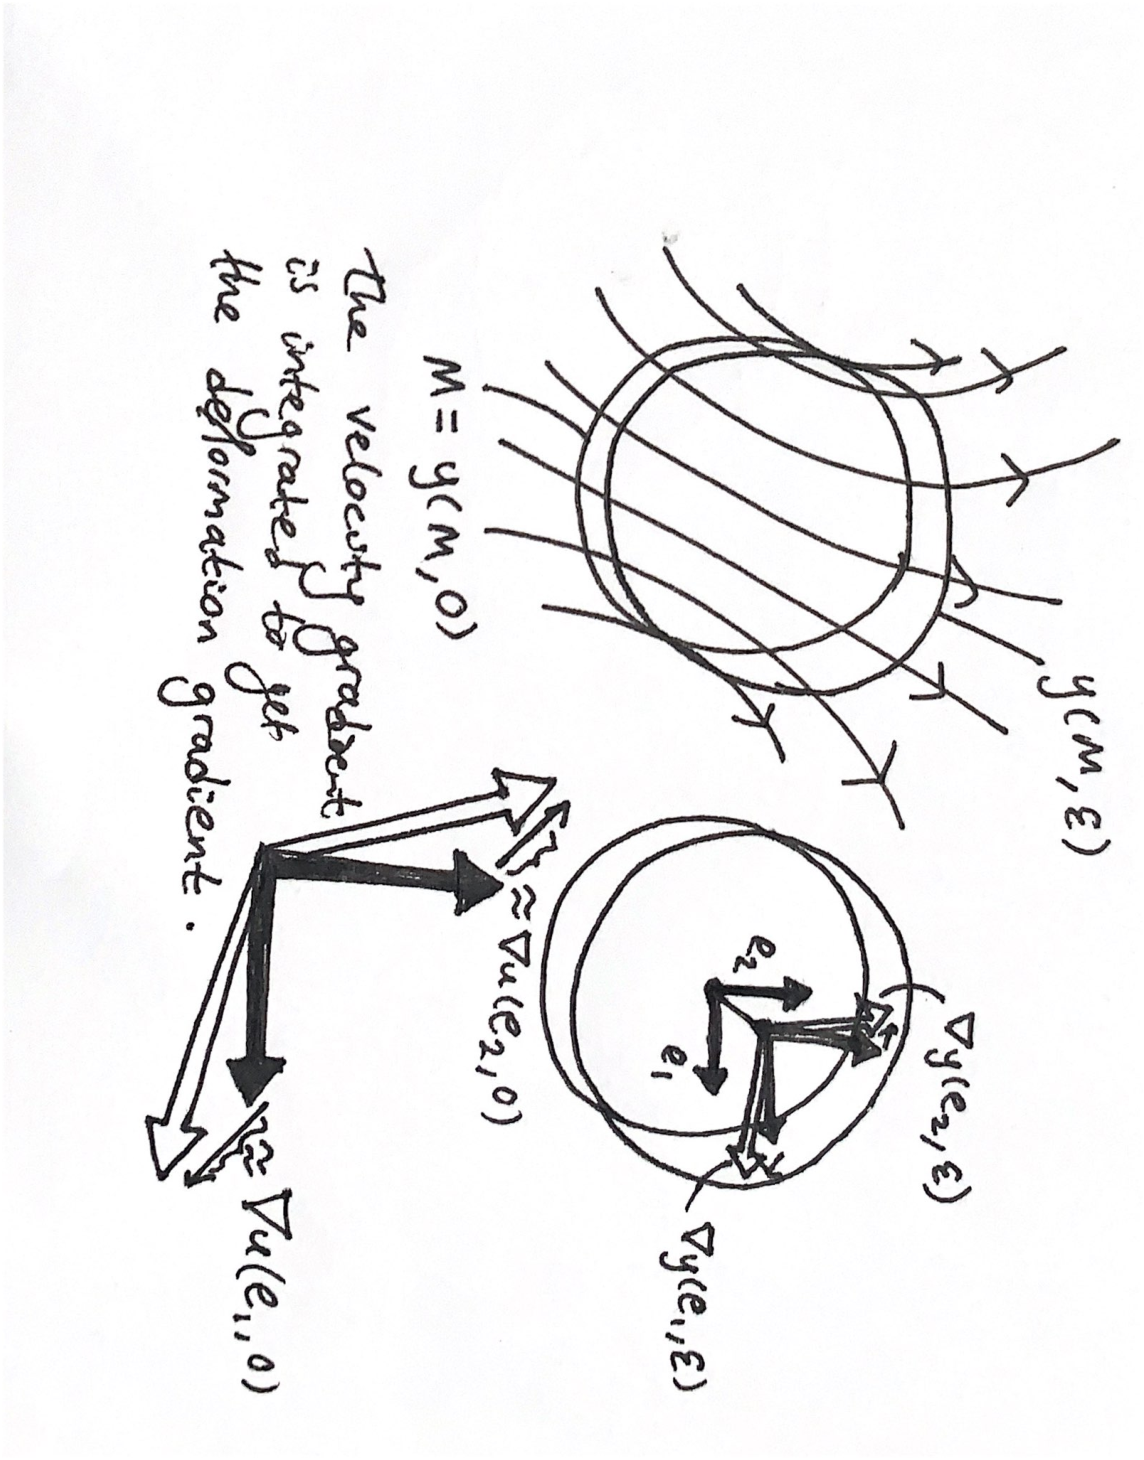
\includegraphics[angle=90,page=1,width=0.58\linewidth]{figures/1.pdf}}
\caption{\small
    The flow of the initial geometry induces a flow on the deformation gradient.
}
\label{sketch_flow_vis}
\end{figure}
We can see that the term $\nabla u$ is a ``differential generator'' of the deformation gradient.
$\nabla u$ is called the \textit{velocity gradient}.
% Polar decomposition, symmetric and antisymmetric parts.
% >>>
\subsection{Material points and material derivatives}\label{material_points}
% <<<
\subsubsection{The material derivative}

Assuming an non-compressing flux function $u$ which transports quantity $\phi$, the differential form of the Reynolds transport theorem
\eqref{lagrangian_transport_differential} becomes
\begin{equation}
    \Part{\phi}{t} + \nabla\cdot(\phi u) = \Part{\phi}{t} + u\cdot\nabla\phi + \cancel{\phi \nabla\cdot u}.
\end{equation}
We define the \textit{material derivative} to be
\begin{equation}\label{material_derivative}
    \frac{D}{Dt} \coloneqq \Part{}{t} + u\cdot\nabla.
\end{equation}
It is a convention to leave the vector field $u$ implicit, as material derivatives are usually taken with respect to the velocity field.
This derivative \eqref{material_derivative} will turn out to measure ``per-volume'' quantities.

\subsubsection{Pieces of the continuum}
A \textit{material element} is a small piece of a continuum model which evolves with the displacement and flow.
In fluid dynamics this is also called a fluid parcel, although it should not be thought of as an object placed in the fluid, but
rather some tracer such as a non-diffusing dye.
This idealisation is sketched in figure \ref{sketch_material_element}.
\begin{figure}[H]
\centerline{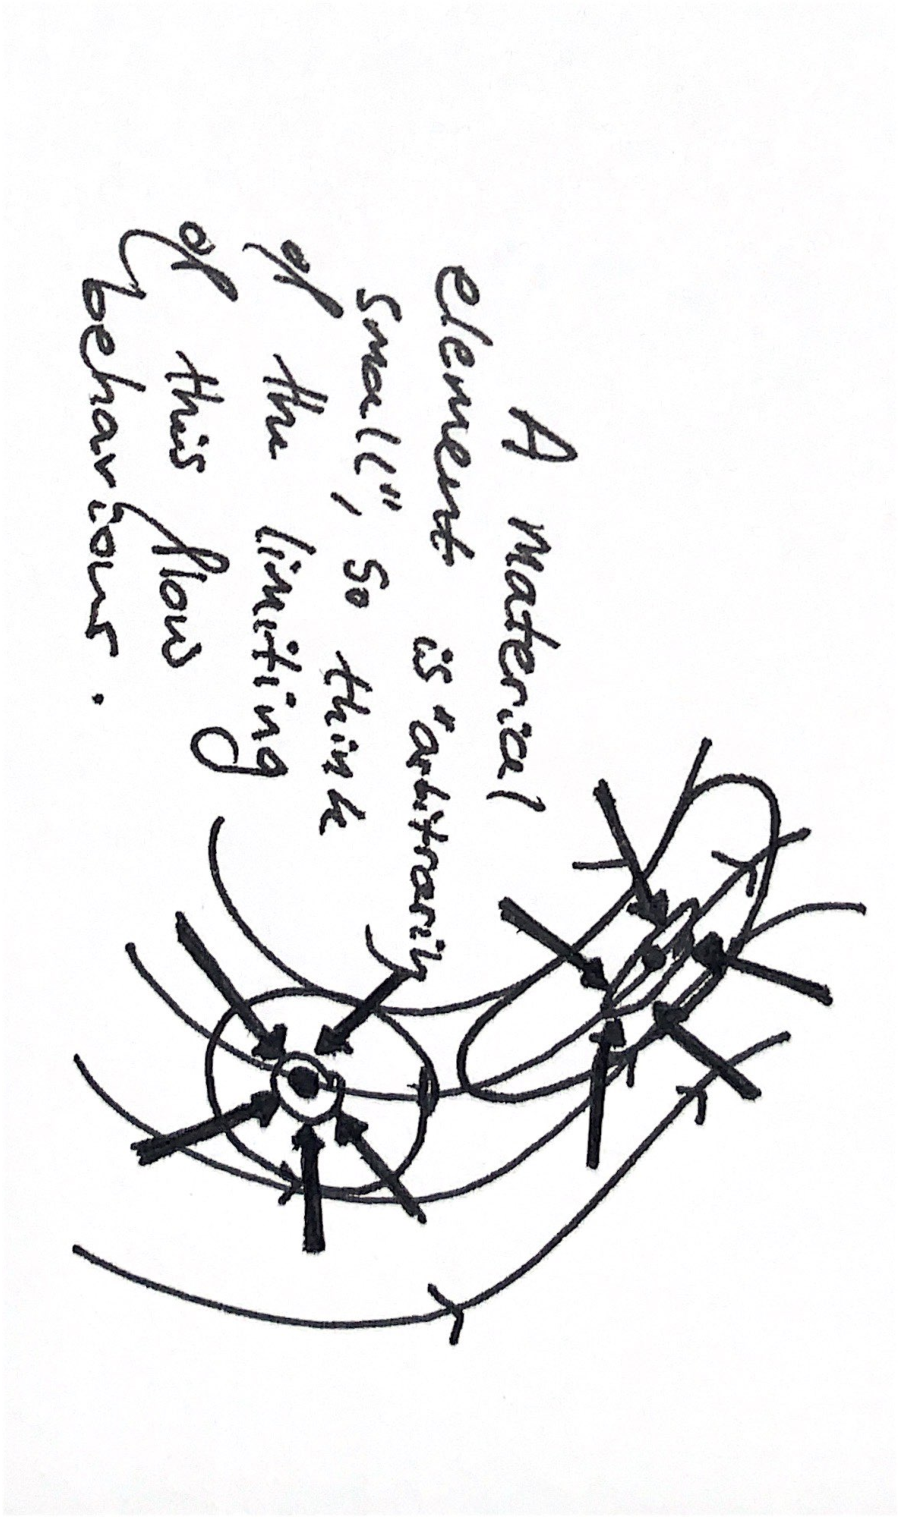
\includegraphics[angle=90,page=1,width=0.55\linewidth]{figures/2.pdf}}
\caption{An idealised material element being pushed by the flow.
    Although the point will not deform under the flow, an ``infinitely small'' material element will.
}
\label{sketch_material_element}
\end{figure}
In continuum mechanics a \textit{material point} is the ideal point of the continuum, corresponding to some macroscopic averaging in physical models.
At a certain point, we can imagine an arbitrarily small fluid parcel being transported by the flow.
No matter how small this is, the parcel will still start to shear, expand, and contract due
to the flow.
The material derivative was defined as $\frac{D}{Dt} \coloneqq \Part{}{t} + u\cdot\nabla$. Notably this derivative contains no divergence term, and so does not
measure the
change of a quantity due to expansion and contraction of the arbitrarily small fluid parcel. Therefore we can think of the material derivative as acting
on \textit{per-volume} quantities.

% \vskip 0.2in
% (figure of a point mass flowing along a scalar field, and a mass with extent being compressed)
% \vskip 0.2in
% \begin{center}
% \includegraphics[page=2,width=0.66\linewidth]{figures/3.pdf}
% \end{center}

% >>>
% >>>

\section{The dynamics of the continuum}
% <<<
\subsection{Conservation of mass}
% <<<
We will take for granted that there is some initial mass density function $\rho_0:M\rightarrow \mathbb{R}^+$
which we would like to conserve.
\subsubsection{The Lagrangian form of mass conservation}
As the position map $y$ evolves, for example under the action of Eulerian velocity field $u$ in the ODE \eqref{position_map_ode},
we would like a mass density function $\rho : N \rightarrow \mathbb{R}^+$ to be greater if the position map ``compresses'' the material,
and smaller if it ``stretches'' the material. Our aim is that the total mass measured in a control volume of $N$ is the same as in its initial configuration.
We can express this by the integral equation
\begin{equation}\label{lagrangian_mass_conservation}
    \int_{\omn} \rho_0(x)\,dx = \int_{y(\omn, t)} \rho(y, t)\,dy,
\end{equation}
where $y(\omn, t)$ denotes the domain pushed forward by the position map. By the usual change of variables formula we have
\begin{equation}\label{lagrangian_mass_conservation_cov}
    \int_{\omn} \rho_0(x)\,dx = \int_{\omn} \det(\nabla y)\rho(y(x,t), t)\,dx,
\end{equation}
where $J = \det(\nabla y)$ is the Jacobian, measuring the local change in the volume element due to the change of variables.
As \eqref{lagrangian_mass_conservation_cov} must hold identically for all $\Omega_0$, we have the localised conservation law
\begin{equation}\label{lagrangian_mass_conservation_local}
    \rho_0 = \det(\nabla y)\rho.
\end{equation}

\subsubsection{The Eulerian form of mass conservation}
Conservation law \eqref{lagrangian_mass_conservation_local} is simple. However, it is given in terms of absolute deformation gradient $\nabla y$.
Instead of asking how mass is distributed
in comparison to its initial configuration, we can ask how mass is transported by $u$.
This gives an instance of the continuity equation \eqref{continuity_equation}, where we have no source:
\begin{equation}\label{eulerian_mass_conservation}
    \frac{d}{dt} \int_{\omn} \rho \,dx + \int_{\pomn} \rho u\cdot \hat{n}\,dx = 0.
\end{equation}
With application of Stokes' theorem we have
\begin{equation}\label{eulerian_mass_conservation_local}
    \Part{\rho}{t} + \nabla \cdot (\rho u) = 0.
\end{equation}
Following \cite{leal}, there is a more geometrical statement of this equation, which will be useful when
we discuss ``material points''
By a divergence product rule \eqref{eulerian_mass_conservation_local} is equivalent to
\begin{equation}\label{eulerian_mass_conservation_local_material}
    \Part{\rho}{t} + u\cdot\nabla\rho + \rho\nabla\cdot u = 0
    \quad\Rightarrow\quad \frac{D\rho}{Dt} = -\rho\nabla\cdot u,
\end{equation}
where $\frac{D}{Dt}$ is the material derivative as defined in \eqref{material_derivative}.

% >>>
\subsection{Conservation of linear momentum}
% <<<
If we conserve the linear momentum $\rho u$, a ``quantity of motion'', under the flow of $u$, then we get a continuity equation
\begin{equation}\label{cauchy_continuity_traction}
    \frac{d}{dt}\int_{\Omega_0(t)}\rho u\,dx = \int_{\omn(t)} \rho g\,dx + \int_{\pomn(t)}\hat{t}\,dx,
\end{equation}
a specific realisation of the Lagrangian continuity equation \eqref{lagrangian_transport}. The Lagrangian perspective is convenient
as it allows us to separate interior and boundary forces on a moving piece of material. The term $g$ is a regular body force per unit mass, where $\rho g$ corresponds to
the source term $s$ in \eqref{lagrangian_transport}. The boundary term involving $\hat{t}$, however, has no analogue in the scalar continuity equation
\eqref{lagrangian_transport}.
This vector term $\hat{t}$ is called the \textit{traction} in continuum mechanics, and measures a local force exerted across the boundary
of the control volume due to the immediately adjacent material.

\subsubsection{The Euler-Cauchy stress principle}\label{stress_principle}
Clearly, in accord with Newton, we would like that two $\Omega_0$ and $\Omega_0^\prime$
which share a boundary element should have equal and opposite tractions across that boundary element.
Since the normal $\hat{n}$ represents a boundary element, and is negative for the opposite element, if $\hat{t}$ is linear in $\hat{n}$ we have this required
property. We can then let \eqref{cauchy_continuity_traction} become
\begin{equation}\label{cauchy_continuity}
    \frac{d}{dt}\int_{\Omega_0(t)}\rho u\,dx = \int_{\omn(t)} \rho g\,dx + \int_{\pomn(t)}\sigma:\hat{n}\,dx
\end{equation}
where $\sigma$ is termed the \textit{Cauchy stress tensor}.
This is the integral form of the \textit{Cauchy momentum equation}, the standard
form of $F = ma$ in continuum mechanics.


% <<<
\subsubsection{Differentializing the Cauchy momentum equation}
By application of the Reynolds transport theorem \eqref{reynolds_transport_theorem_tensor} to \eqref{cauchy_continuity} we get
\begin{equation}\label{cauchy_continuity_eulerian}
    \int_{\Omega_0(0)}\Part{(\rho u)}{t}\,dx + \int_{\partial\Omega_0(0)}\rho u (u\cdot \hat{n})\,dx = \int_{\Omega_0(0)} \rho g\,dx + \int_{\pomn(0)} \sigma:\hat{n}\,dx.
\end{equation}
Differentializing \eqref{cauchy_continuity_eulerian}, by our previously derived tensor identities, gives
\begin{equation}\label{cauchy_continuity_differential}
    \Part{(\rho u)}{t} + \nabla \cdot (\rho u\otimes u) = \rho g + \nabla\cdot\sigma.
\end{equation}
This is called the \textit{conservative form} of the Cauchy momentum equation.
We can derive another, possibly more convenient form of \eqref{cauchy_continuity_differential} using the fact that
$\rho$ is conserved and has no source. Here, this will be derived purely algebraically, although the final form of the equation
has a useful interpretation. Expanding the partial derivative
$$
    \Part{(\rho u)}{t} = \rho\Part{u}{t} + u\Part{\rho}{t}
$$
is simple. The tensor divergence $\nabla \cdot (\rho u\otimes u)$ is defined such that
$$
    \int_{\Omega_0} \nabla \cdot (\rho u\otimes u)\,dx = \int_{\pomn} (\rho u\otimes u) : \hat{n}\,dx = \int_{\pomn} \rho u (u\cdot\hat{n})\,dx
$$
for arbitrary control volumes $\Omega_0$. As $\Omega_0$ becomes small, we can separately assume $u$ and $\rho u$ are constant
to derive
$$
    \int_{\pomn} \rho u (u\cdot\hat{n})\,dx = u\int_{\pomn}(\rho u)\cdot\hat{n}\,dx
                                              + \rho u\cdot \int_{\pomn} u\hat{n}\,dx \quad+\quad\cdots
$$
where a trailing term becomes neglible for a small control volume. This gives a ``tensor product rule'' for the divergence,
\begin{equation}\label{cauchy_divergence_tensor_product}
    \nabla\cdot (\rho u \otimes u) = u\nabla\cdot (\rho u) + \rho u\cdot\nabla u.
\end{equation}
Equation \eqref{cauchy_continuity_differential} then becomes
$$
    \rho\Part{u}{t} + u\Part{\rho}{t} + u\nabla\cdot (\rho u) + \rho u\cdot\nabla u = \rho g + \nabla\cdot\sigma.
$$
Noting that $\Part{\rho}{t}$ is already given by continuity equation \eqref{eulerian_mass_conservation_local}
$$\Part{\rho}{t} = -\nabla\cdot(\rho u),$$
as mass is transported by $u$ and has no source, we get
$$
    \rho\Part{u}{t} -\cancel{u\nabla(\rho u)} + \cancel{u\nabla\cdot (\rho u)} + \rho u\cdot\nabla u = \rho g + \nabla\cdot\sigma.
$$
Finally, the material derivative, as defined in section \ref{material_points}, is helpful in simplifying the above to
\begin{equation}\label{cauchy_continuity_differential_material}
    \rho\frac{Du}{Dt} = \rho g + \nabla\cdot\sigma.
\end{equation}
This form of \eqref{cauchy_continuity_differential} is called the \textit{convective form} of the Cauchy momentum equation, and is more obviously a form of $F = ma$.
% From this derivation we have the identity
% \begin{equation}\label{mass_conserved_linear_momentum_identity}
%     \Part{(\rho u)}{t} + \nabla\cdot(\rho u\otimes u)
%     = \rho\frac{Du}{Dt}
% \end{equation}
% when mass density $\rho$ is conserved by $u$. The left-hand-side in \eqref{mass_conserved_linear_momentum_identity} is the differentialized Reynolds transport \eqref{reynolds_transport_theorem_tensor_differential},
% which measures the change in total linear momentum when following a small control volume that begins at a point $x^*$ and flows with $u$.
% If we integrate both sides over a control volume and apply the Reynolds transport theorem, we get
% \begin{equation}\label{mass_conserved_linear_momentum_identity_integral}
%     \eval{\frac{d}{dt}\left[\int_{\omn(t)} \rho u\,dx\right]}_{t=0} = \int_{\omn(0)} \rho \frac{Du}{Dt}\,dx.
% \end{equation}
% >>>
Recall that the material derivative is defined as
    $$\frac{D}{Dt} \coloneqq \Part{}{t} + u\cdot \nabla,$$
which measures the rate of change of a pointwise quantity from the perspective of a particle moving with the flow field $u$.
The equation \eqref{cauchy_continuity_differential_material} then says that, if the continuum consists of idealised points
each with a certain linear momentum (in the particle sense), deflection of their inertial path is due only to the application
of a body force $\rho g$ at this point, and a total traction force exerted by the surrounding material.
% >>>
\subsection{Constitutive relations}\label{constitutive_relations}
% <<<
The conservation equations derived are conservation of mass \eqref{eulerian_mass_conservation_local} and conservation of linear momentum \eqref{cauchy_continuity_differential_material}.
Here the equations are given in their typical differential form for flow problems, with the Eulerian perspective of mass conservation, and the
convective form of linear momentum conservation:
\begin{equation}\label{conservation_system}
\begin{split}
    \frac{D\rho}{Dt} + \rho\nabla\cdot u = 0 &\quad\text{(Conservation of mass)},
    \\
    \rho\frac{Du}{Dt} = \rho g + \nabla\cdot\sigma &\quad\text{(Conservation of linear momentum)}.
\end{split}
\end{equation}
The unknowns include mass density $\rho$ and velocity $u$, described by $1 + d$ scalar functions where $d$ is the dimension of the domain.
We can see there are $1 + d$ equations by expanding $u$ in terms of components in some basis.
\begin{align*}
\begin{split}
    \rho\frac{Du_i}{Dt} = \rho g_i + \left(\nabla\cdot\sigma\right)_i &\quad\text{(Conservation of linear momentum components)},
    \\
    i=1,\cdots,d. &
\end{split}
\end{align*}
When $g$ and $\sigma$ are known, where $\sigma$ is not determined by the material state, this system is well-formed, but not very interesting.
This effectively models a continuum of non-interacting material points, with a linear-momentum-introducing source function $\rho g + \nabla\cdot \sigma$.
However, we usually let $g$ be known (as this is a per-mass external body force, for example gravity), and the Cauchy stress tensor $\sigma$ be unknown,
to be determined by the material state.
This gives $d^2$ more unknowns, so the system is heavily underdetermined. In effect, the system \eqref{conservation_system} is
underdetermined because we don't have a specific material in mind.

\subsubsection{Constitutive relations}
A specification of the Cauchy stress tensor $\sigma$ is called a \textit{constitutive relation},
as $\sigma$ depends on the ``material constitution''.
A constitutive relation specifies how the material configuration
induces forces on the material, or rather, how kinematics is related to dynamics. With $\sigma$ specified, the Cauchy momentum equation \eqref{cauchy_continuity_differential_material} becomes well-posed
(however, in general, $\sigma$ may depend on new variables such as temperature, requiring further equations).

% \subsubsection{Deviatoric and volumetric stresses}
% Suppose that the tractions are determined only by the velocity gradient,
%     $$\sigma = \sigma(\nabla u).$$
% We have the symmetric-antisymmetric splitting of the velocity gradient
% \newcommand{\usym}{\frac{1}{2}\left(\nabla u + \nabla u^T\right)}
% \newcommand{\uantisym}{\frac{1}{2}\left(\nabla u - \nabla u^T\right)}
% \begin{align*}
%     \nabla u = \usym + \uantisym.
% \end{align*}
% The symmetric term $\usym$ can be thought of as differential generator of stretching (as the exponential of a symmetric matrix is symmetric-positive-definite),
% and the antisymmetric term $\uantisym$ can be thought of as a differential generator of rotations (as the exponential of an antisymmetric matrix is orthogonal).

% \subsubsection{Pressure in incompressible materials}
% TODO: Shorten or remove
% 
% 
% The concept of pressure will be very important in our discussion of the Navier-Stokes equations, so we introduce it
% here. A detailed derivation of the pressure is given in terms of Stokes flow in section \ref{pressure_derivation}.
% 
% If we require the velocity field $u$ of the position map $x$ to be non-compressing (as described in section (ref)),
% then we add to our model equations the constraint
% \begin{equation}\label{noncompressing_velocity}
%     \nabla \cdot u = 0.
% \end{equation}
% We proceed by analogy to a simple mechanical system.
% The state of a pendulum of mass $m$ might be described by two spatial variables $X$ and $Y$ with a constraint
%     $$X^2 + Y^2 = 1.$$
% Given a differentiable pendulum motion, the linear momenta $mv_X$ and $mv_Y$ clearly cannot be constant, as then the pendulum
% would ``fly out'' of its arc.
% From the perspective of the $X,Y$ coordinate system there exists ``virtual forces'' which are exactly those that are needed
% to maintain constraints. These forces have no necessary physical interpretation, as the pendulum model does not explicitly reference
% the tension of the pendulum rod, but are rather those strong forces that must ``come from somewhere'' such that the constraints
% are satisfied.
% 
% \vskip 0.2in
% (figure)
% \vskip 0.2in
% 
% From a constraint on position $(X,Y)$ we can derive a constraint on velocity $(v_X,v_Y)$ by noting that the velocity must stay inside
% the tangent plane in the configuration space. In this case, we require
% \begin{equation}\label{pendulum_velocity_constraint}
%     Xv_X + Yv_Y = 0.
% \end{equation}
% (--- add Lagrange multipliers to the system, then pressure here is a sort of Lagrange multiplier).
% The continuum velocity constraint \eqref{noncompressing_velocity} is completely analogous to \eqref{pendulum_velocity_constraint}.
% Motions of $x$ are restricted to those which do not compress mass. Clearly, our (per-point) linear momentum $\rho u$
% cannot be constant except in simple parallel flows, implying the existence of some virtual (per-point) force.
% We call this force the \textit{pressure} $p$, and we are now solving for $\rho$, $u$, and $p$ in a coupled system of equations
% \eqref{cauchy_continuity_differential_material} and \eqref{noncompressing_velocity}, repeated here:
% \begin{align*}
%     \rho\frac{Du}{Dt} = \rho g + \nabla\cdot\sigma,\quad
%         \nabla \cdot u = 0.
% \end{align*}
% As there is no explicit mention of $p$, it must be part of the constitutive relation for $\sigma$.
% We let $\sigma$ be
% \begin{align*}
%     \sigma = -pI + \tau \quad\Rightarrow\quad \nabla\cdot\sigma = -\nabla p + \nabla\cdot \tau,
% \end{align*}
% where $I$ is the identity tensor and $\tau$ is called the \textit{deviatoric} component of the Cauchy stress tensor.
% $\tau$ is chosen such that the pressure $p$ entirely encapsulates the isotropic forces which push material volumes apart.

\subsubsection{Completing the equations}
We have so far been working quite generally with the forms of continuum mechanics models and their constraints. Although we have made some assumptions
(for example, we require $\sigma$ to be a purely a function of the local linearisation of the continuum model, an idealisation due to Cauchy), we must so far leave
our systems underdetermined.
In the next chapter, we will
investigate an important constitutive relation for the stress $\sigma$, forming what is called a \textit{Navier-Stokes fluid},
giving a complete system of equations called the \textit{Navier-Stokes equations}.
% >>>
% >>>
